\documentclass[a4paper]{article}

\usepackage[english]{babel}
\usepackage[utf8]{inputenc}
\usepackage{amsmath}
\usepackage{graphicx}
\usepackage[breaklinks]{hyperref}
\usepackage{caption}

\title{
	Project 02 \\
	\bigskip
	\normalsize APSC 607 Fall 2017
}

\author{Seth Goodman}

\date{\today}

\begin{document}
\maketitle


%\begin{abstract}
%\end{abstract}

\section{Introduction}
\label{sec:introduction}


This project explored methods for calculating the integral roots of functions. Each functions was  examined in the range between zero and two, using the Composite Trapezoidal Rule, Composite Midpoint Rule, Composite Simpson’s Rule, as well as an adaptive implementation of the Composite Simpson’s Rule. The behavior and characteristics of these methods are reviewed by examining the effectiveness of the resulting value for the integral given a range of values for N. 

All computations were performed using MATLAB using the code (Table 1) accompanying this report (in a zip file). The following Methods section will present the methods used in MATLAB to explore functions, as well as the outputs and results. The Results section of this report contains the outputs for each function and range along with related observations and discussion. All figures and tables found in this report are available in the output subdirectory of the accompanying zip file. Additionally, all code and figures found in the zip file can be accessed via GitHub\footnote{\url{https://github.com/sgoodm/apsc607/tree/master/project_02}}.



\newpage
\section{Methods}
\label{sec:methods}

True integral calculated using MATLAB built in symbolic and numeric methods

Overview of methods



\subsection{Composite Trapezoidal Rule}
TEXT

\begin{center}
	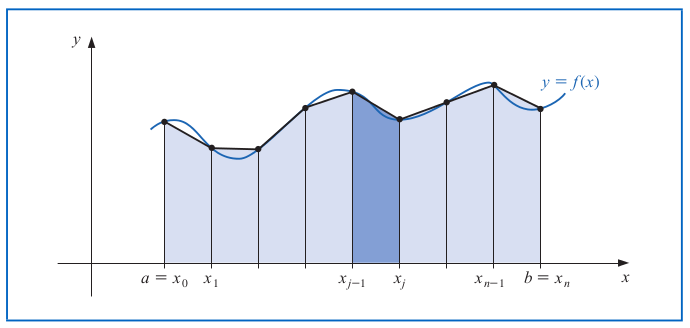
\includegraphics[width=1\textwidth]{../additional/trapezoidal_fig.png}
	\captionof{figure}{Trapezoidal Figure\cite{burden2010}}
	\label{trap_fig}
\end{center}


The Composite Trapezoidal Rule for $n$ intervals, as seen in Figure \ref{trap_fig}, can be defined by Equation \ref{trap_eq}, given $h=(b-a)/n$ and $x_j=a+jh$, for each $j=0,1,\dots,n$\cite{burden2010}.

\begin{equation}
\int_{a}^b f(x) dx = \frac{h}{2} \Bigg[ f(a) + 2 \sum_{j=1}^{n-1} f(x_j) + f(b) \Bigg]
\label{trap_eq}
\end{equation}

Implementing this in a MATLAB function is extremely straightforward. The function accepts a function handle \textbf{f} defining $f(x)$, (e.g., $cos(x)$), the desired number of internval \textbf{n}, along with our bounds \textbf{rmin} and \textbf{rmax}. The value for \textbf{h} given \textbf{n} is calculated, as are the vectors \textbf{j} and \textbf{$x_j$}. Using these components and the summation function, the final integral for the input conditions can be calculated. The function then returns the integral value, along with the value of \textbf{h} used.

This function implementing the Trapezoidal Rule for integration (as well as subsequent Midpoint and Simpson's Rules) is called over a range of values for \textbf{n} using the \textbf{arrayfun} function in MATLAB. This function accepts another function, defining our integration rule, and a vector, and simply repeatedly calls the specified value while iterating over the values in the vector. The call to \textbf{arrayfun} then return a vector (or set of vectors in this case) containg the results from each call to the integration function.

 The resulting vector of integral values across varying \textbf{n} can compared with the true integral value generated earlier, to produce an error vector. The error vector is used to identify the value of \textbf{n} (and thus \textbf{h}) at which the integration rule produced results that were accurate within a desired tolerance.



\subsection{Composite Midpoint Rule}
TEXT

\begin{center}
	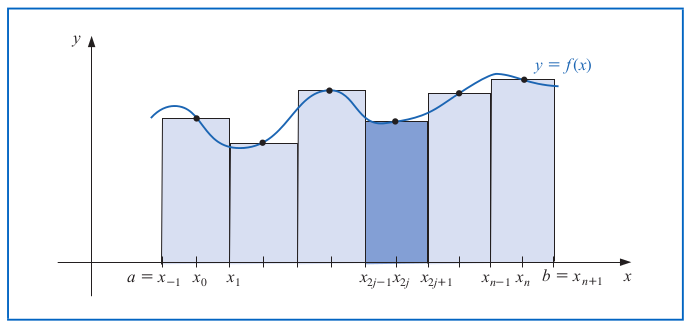
\includegraphics[width=1\textwidth]{../additional/midpoint_fig.png}
	\captionof{figure}{Midpoint Figure\cite{burden2010}}
	\label{mid_fig}
\end{center}

The Composite Midpoint Rule for $n+2$ intervals, as seen in Figure \ref{mid_fig}, can be defined by Equation \ref{mid_eq}, given $h=(b-a)/(n+2)$ and $x_j=a+(j+1)h$, for each $j=-1,0,\dots,n+1$\cite{burden2010}.

\begin{equation}
\int_{a}^b f(x) dx = 2h \sum_{j=0}^{n/2}f(x_2j)
\label{mid_eq}
\end{equation}

\subsection{Composite Simpson's Rule}
TEXT

\begin{center}
	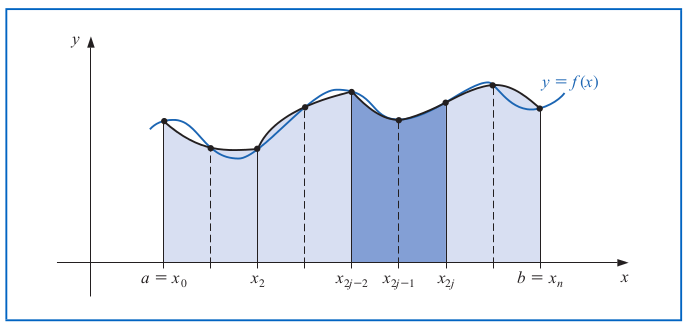
\includegraphics[width=1\textwidth]{../additional/simpsons_fig.png}
	\captionof{figure}{Simpson's Figure\cite{burden2010}}
	\label{sim_fig}
\end{center}

The Composite Simpson's Rule for $n$ intervals, as seen in Figure \ref{sim_fig}, can be defined by Equation \ref{sim_eq}, given $h=(b-a)/n$ and $x0_j=a+jh$, $x1_j=a+jh+h/2$, $x2_j=a+jh+h$,  for each $j=0,1,\dots,n-1$.
 
    
\begin{equation}
\int_{a}^b f(x) dx = \sum_{j=0}^{n-1} \Bigg[ \frac{h}{6} \big[ f(x0_j) + 4f(x1_j) + f(x2_j) \big] \Bigg]
\label{sim_eq}
\end{equation}



\subsection{Adaptive Simpson's Rule}
TEXT



\newpage
\section{Results}
\label{sec:results}

TEXT

Error comparison

\begin{equation}
\frac{b-a}{6}h^2f^{''}(u)
\label{trap_err}
\end{equation}

\begin{equation}
\frac{b-a}{12}h^2f^{''}(u)
\label{mid_err}
\end{equation}

\begin{equation}
\frac{h^5}{90}f^{(4)}(\xi_j)
\label{sim_err}
\end{equation}
  


\begin{enumerate}
\item Like this,
\item and like this.
\end{enumerate}

\begin{itemize}
\item Like this,
\item and like this.
\end{itemize}

\begin{description}
\item[Word] Definition
\item[Concept] Explanation
\item[Idea] Text
\end{description}

\dots using dots \dots


\begin{equation}
f(x) = e^{2x} * sin(3x)
\label{eq:fa}
\end{equation}

\begin{equation}
f(x) = \frac{1}{x+4}
\label{eq:fb}
\end{equation}



before figure 1a
\begin{center}
	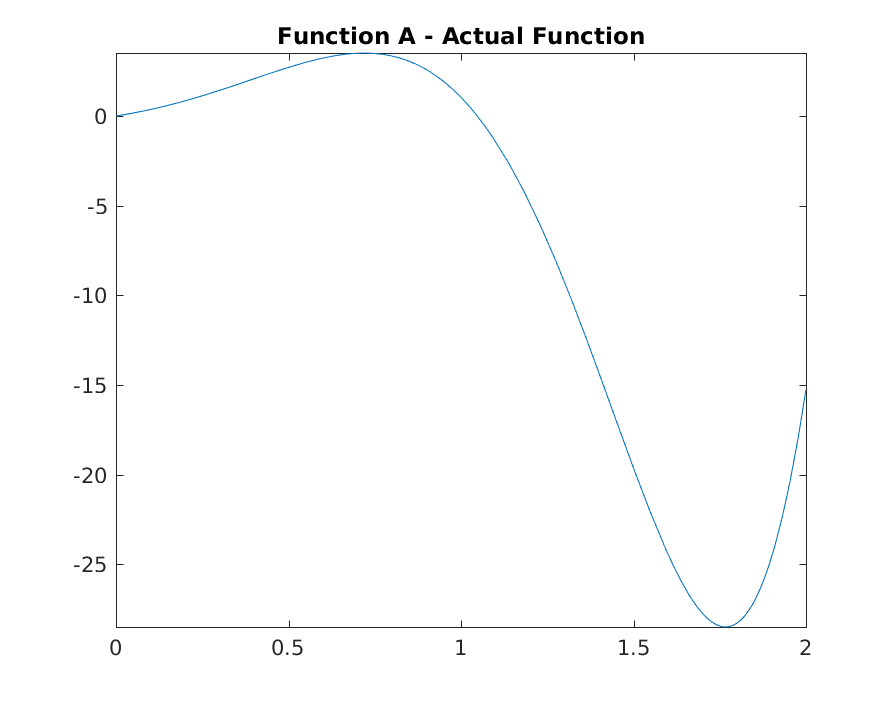
\includegraphics[width=1\textwidth]{../output/a_actual.png}
	\captionof{figure}{caption text a}
	\label{figa}
\end{center}
after figure 1a



\bgroup
\def\arraystretch{1.5}
\begin{center}
	\centering
	\begin{tabular}{l|r}
	\textbf{Item} & \textbf{Quantity} \\
	\hline
	Widgets & 42 \\
	Gadgets & 13
	\end{tabular}
	\captionof{table}{An example table.}
	\label{table1}
\end{center}
\egroup




Something about minimum error in footnote\footnote{See following link on MATLAB precision limitions (general limitations of floating point representations apply) https://www.mathworks.com/help/fixedpoint/ug/limitations-on-precision.html}.




\newpage
\begin{thebibliography}{9}
\bibitem{burden2010}
  Burden, R., Faires, J., Numerical Analysis 9th Edition. 2010

\end{thebibliography}
\end{document}
